\documentclass[12pt,a4paper]{article}

% Font and Vietnamese support
\usepackage{fontspec}
\setmainfont{Times New Roman}

% Page layout
\usepackage[margin=2.5cm]{geometry}
\usepackage{setspace}
\onehalfspacing

% Tables
\usepackage{booktabs}
\usepackage{tabularx}

% Graphics and floats
\usepackage{graphicx}
\usepackage{float}

% Links
\usepackage[colorlinks=true,linkcolor=blue,urlcolor=blue]{hyperref}

% Lists
\usepackage{enumitem}

% Paragraph formatting
\setlength{\parindent}{0pt}
\setlength{\parskip}{0.8em}

\begin{document}

% ==================== TRANG BÌA ====================
\begin{titlepage}
\centering
\vspace*{4cm}

{\Huge\bfseries Demo RunPod Flash\par}
\vspace{0.5cm}
{\Large Speech-to-Text Deployment trên Serverless GPU\par}

\vspace{3cm}

{\large
\begin{tabular}{rl}
\textbf{Người thực hiện:} & Nguyễn Hải Thiện \\[6pt]
\textbf{Thời gian:} & 14:00, ngày 02/07/2026 \\[6pt]
\textbf{GitHub:} & \url{https://github.com/adamwhite625/demo-runpod-stt} \\[6pt]
\textbf{Web Demo:} & \url{https://demo-runpod-stt.streamlit.app/} \\
\end{tabular}
}

\vfill
\end{titlepage}

% ==================== MỞ ĐẦU ====================
\section*{Mở đầu}

Báo cáo này trình bày kết quả demo hệ thống Speech-to-Text (STT) được triển khai trên nền tảng RunPod Flash, phục vụ cho bài toán Voice Bot Call Center. Mục tiêu gồm hai phần: (1) đo lường hiệu năng thực tế của mô hình faster-whisper trên GPU cloud, và (2) so sánh hai kiến trúc triển khai serverless (Flash vs Docker) để đưa ra khuyến nghị phù hợp cho từng giai đoạn phát triển sản phẩm.

% ==================== CHƯƠNG 1 ====================
\section{Đánh giá Hiệu năng Speech-to-Text}

\subsection{Cấu hình hệ thống}

\begin{table}[H]
\centering
\begin{tabular}{ll}
\toprule
\textbf{Thành phần} & \textbf{Chi tiết} \\
\midrule
Mô hình & faster-whisper (\texttt{large-v3-turbo}) \\
GPU & NVIDIA RTX A5000 (24GB VRAM) \\
Compute Type & float16 \\
Nền tảng & RunPod Flash Serverless \\
Workers & (0, 1) -- hỗ trợ scale-to-zero \\
Idle Timeout & 5 giây \\
\bottomrule
\end{tabular}
\caption{Cấu hình triển khai}
\end{table}

% ---------- Kịch bản 1: File ngắn ----------
\subsection{Kịch bản 1: Hội thoại ngắn (15.5 giây)}

File test: \texttt{demo\_stt\_small.mp3} (61.6 KB, 15.5 giây). Nội dung mô phỏng cuộc gọi xác nhận đơn hàng giao hàng nhanh. Ngôn ngữ: Tiếng Việt -- Confidence: 100\%.

\begin{figure}[H]
    \centering
    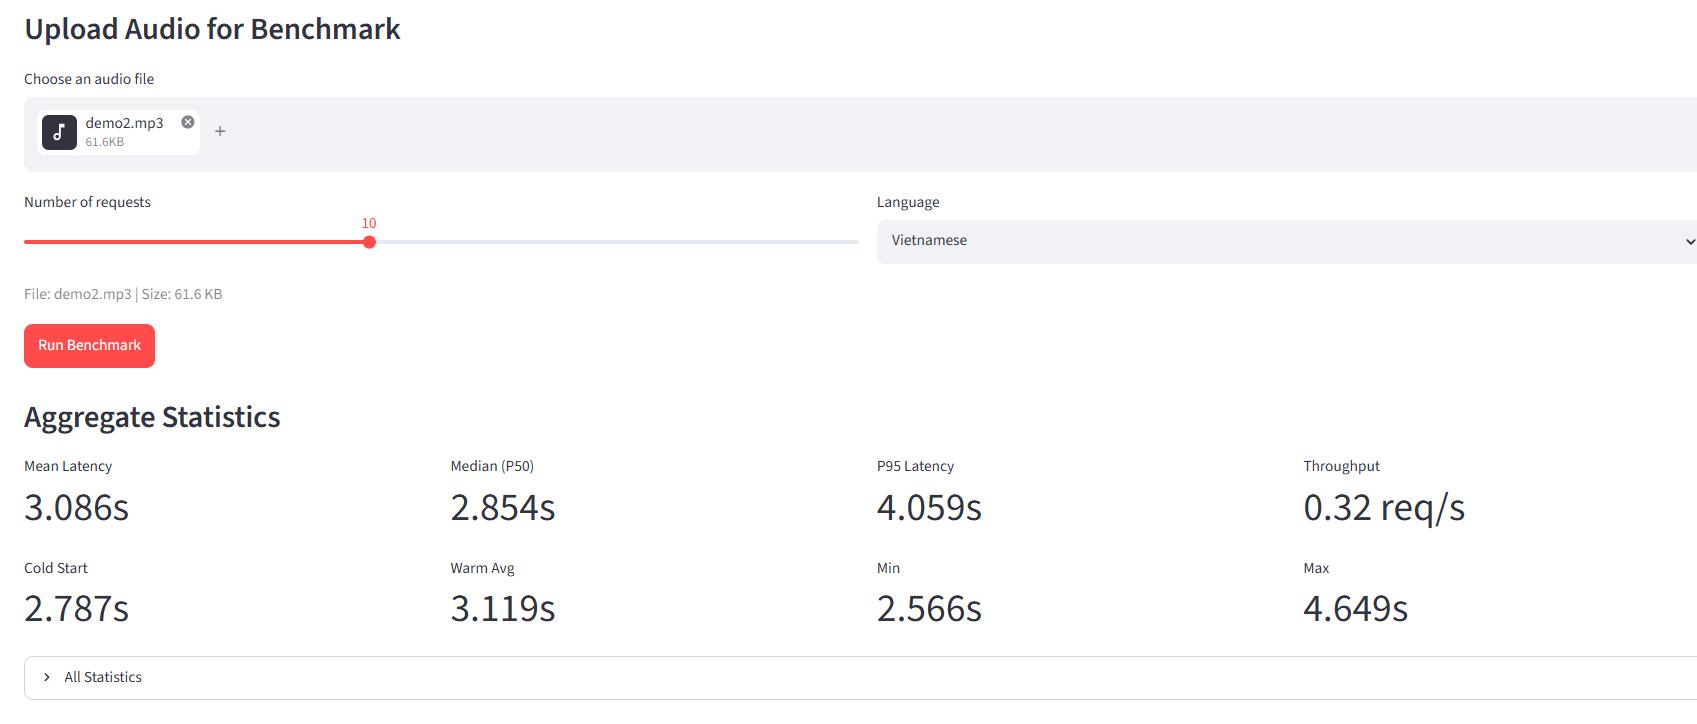
\includegraphics[width=0.9\textwidth]{../images/small/anh1.jpg}
    \caption{Kết quả transcription -- file ngắn}
\end{figure}
\begin{figure}[H]
    \centering
    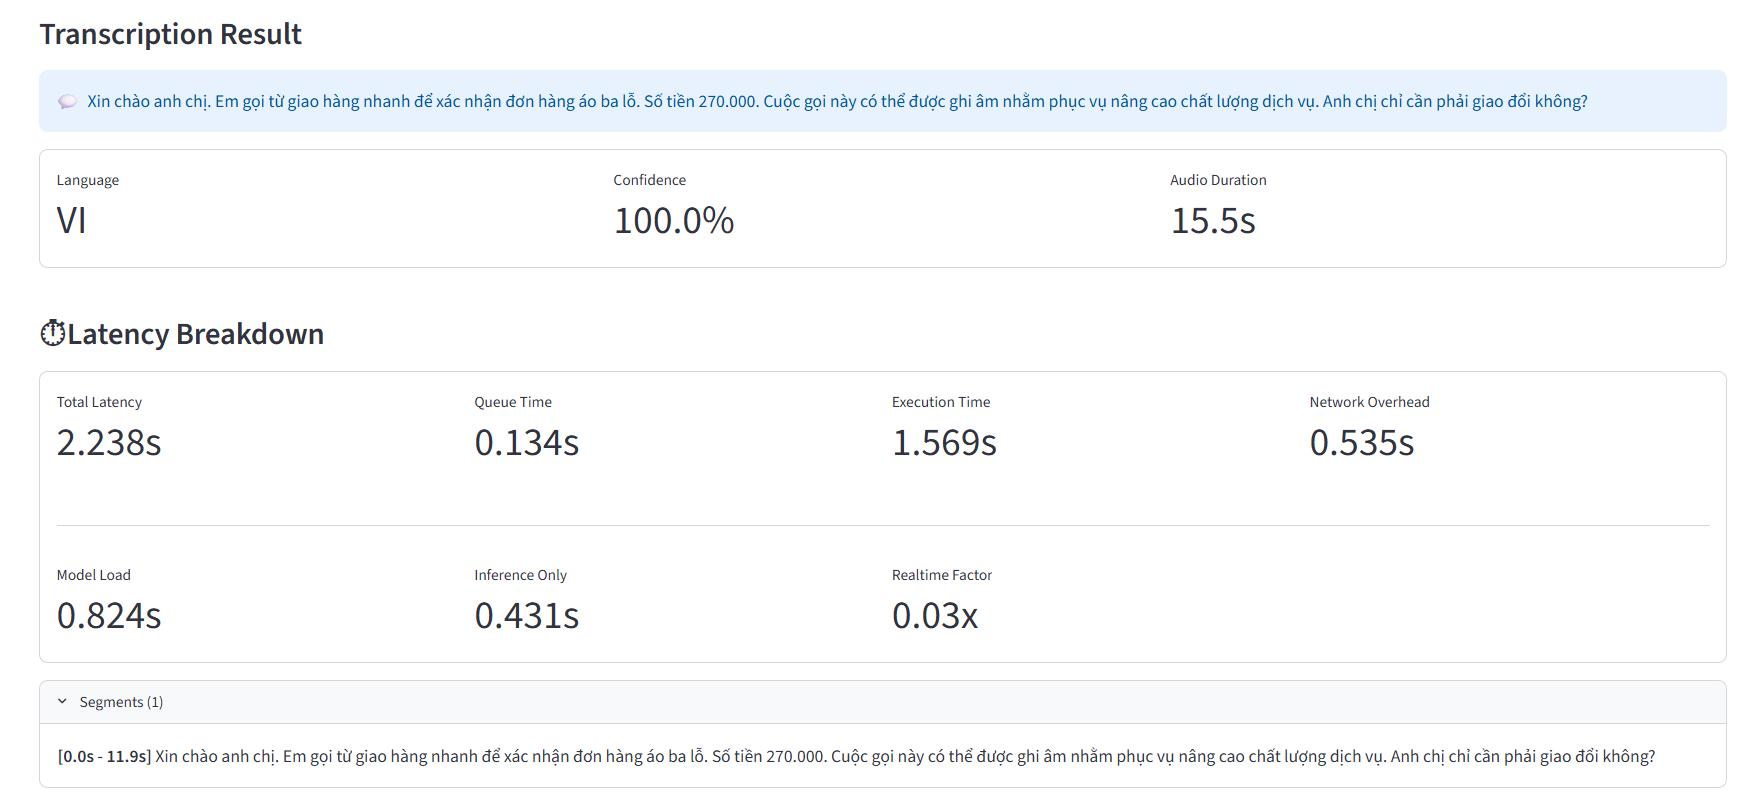
\includegraphics[width=0.9\textwidth]{../images/small/anh2.jpg}
    \caption{Kết quả benchmark -- file ngắn}
\end{figure}
\begin{figure}[H]
    \centering
    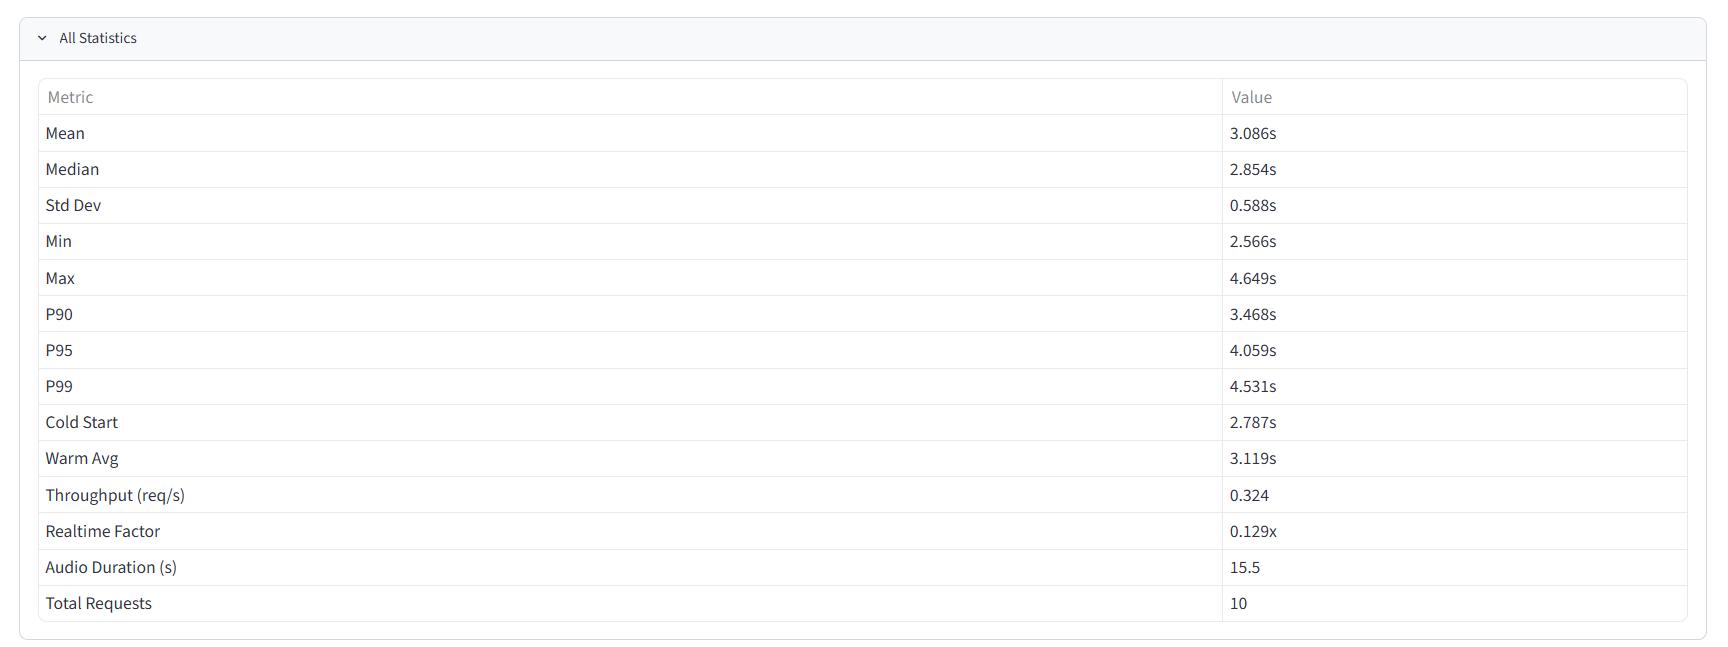
\includegraphics[width=0.9\textwidth]{../images/small/anh3.jpg}
    \caption{Thống kê chi tiết benchmark -- file ngắn}
\end{figure}

\subsubsection{Kết quả request đơn lẻ}

\begin{table}[H]
\centering
\begin{tabular}{lr}
\toprule
\textbf{Chỉ số} & \textbf{Giá trị} \\
\midrule
Total Latency (end-to-end) & 2.238s \\
Queue Time & 0.134s \\
Execution Time & 1.569s \\
Network Overhead & 0.535s \\
\midrule
Model Load & 0.824s \\
Inference Only & 0.431s \\
Realtime Factor (RTF) & 0.03x \\
\bottomrule
\end{tabular}
\caption{Latency breakdown -- file ngắn, single request}
\end{table}

RTF = 0.03x có nghĩa là thời gian inference thực tế (0.431s) chỉ bằng 3\% độ dài audio (15.5s), tương đương tốc độ xử lý nhanh gấp khoảng 33 lần so với thời gian thực.

\subsubsection{Benchmark 10 requests liên tục}

\begin{table}[H]
\centering
\begin{tabular}{lr}
\toprule
\textbf{Chỉ số} & \textbf{Giá trị} \\
\midrule
Mean Latency & 3.086s \\
Median (P50) & 2.854s \\
Std Dev & 0.588s \\
P90 & 3.468s \\
P95 & 4.059s \\
P99 & 4.531s \\
Min / Max & 2.566s / 4.649s \\
\midrule
Cold Start & 2.787s \\
Warm Average & 3.119s \\
Throughput & 0.324 req/s \\
Realtime Factor & 0.129x \\
\bottomrule
\end{tabular}
\caption{Benchmark 10 requests -- file ngắn}
\end{table}



% ---------- Kịch bản 2: File dài ----------
\subsection{Kịch bản 2: Hội thoại dài (79.1 giây)}

File test: \texttt{demo\_stt\_large.mp3} (309.9 KB, 79.1 giây). Nội dung mô phỏng cuộc gọi xử lý khiếu nại giao hàng với nhiều lượt đối thoại. Ngôn ngữ: Tiếng Việt -- Confidence: 100\%.

\begin{figure}[H]
    \centering
    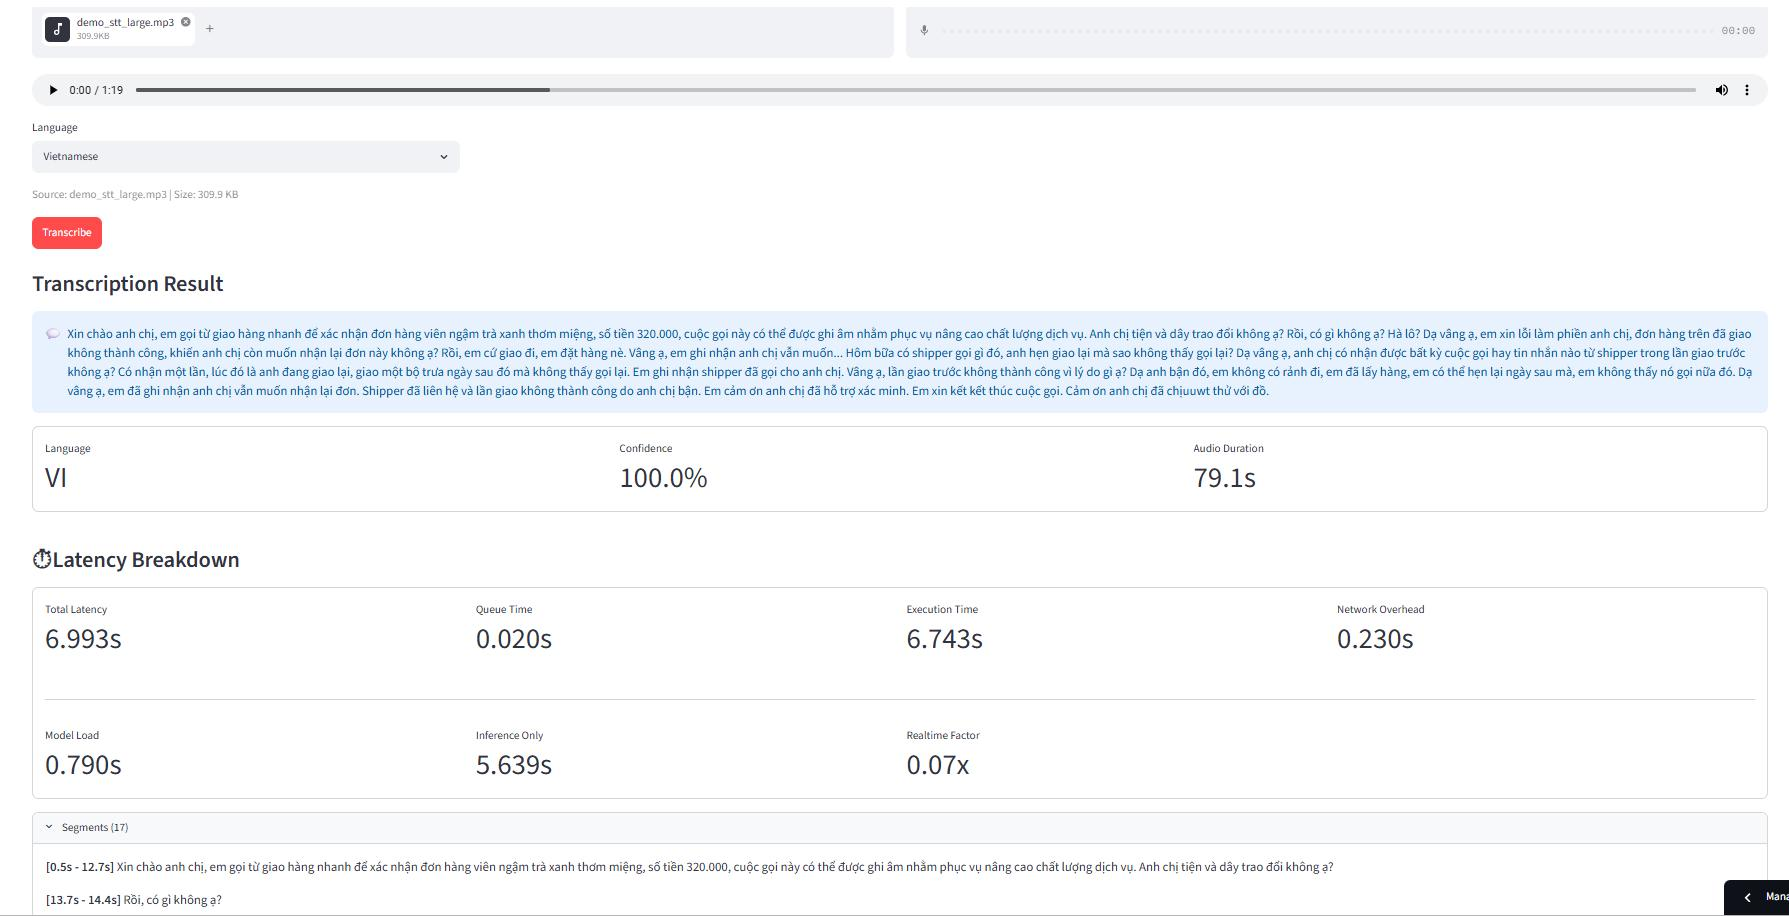
\includegraphics[width=0.9\textwidth]{../images/large/anh1.jpg}
    \caption{Kết quả transcription -- file dài}
\end{figure}
\begin{figure}[H]
    \centering
    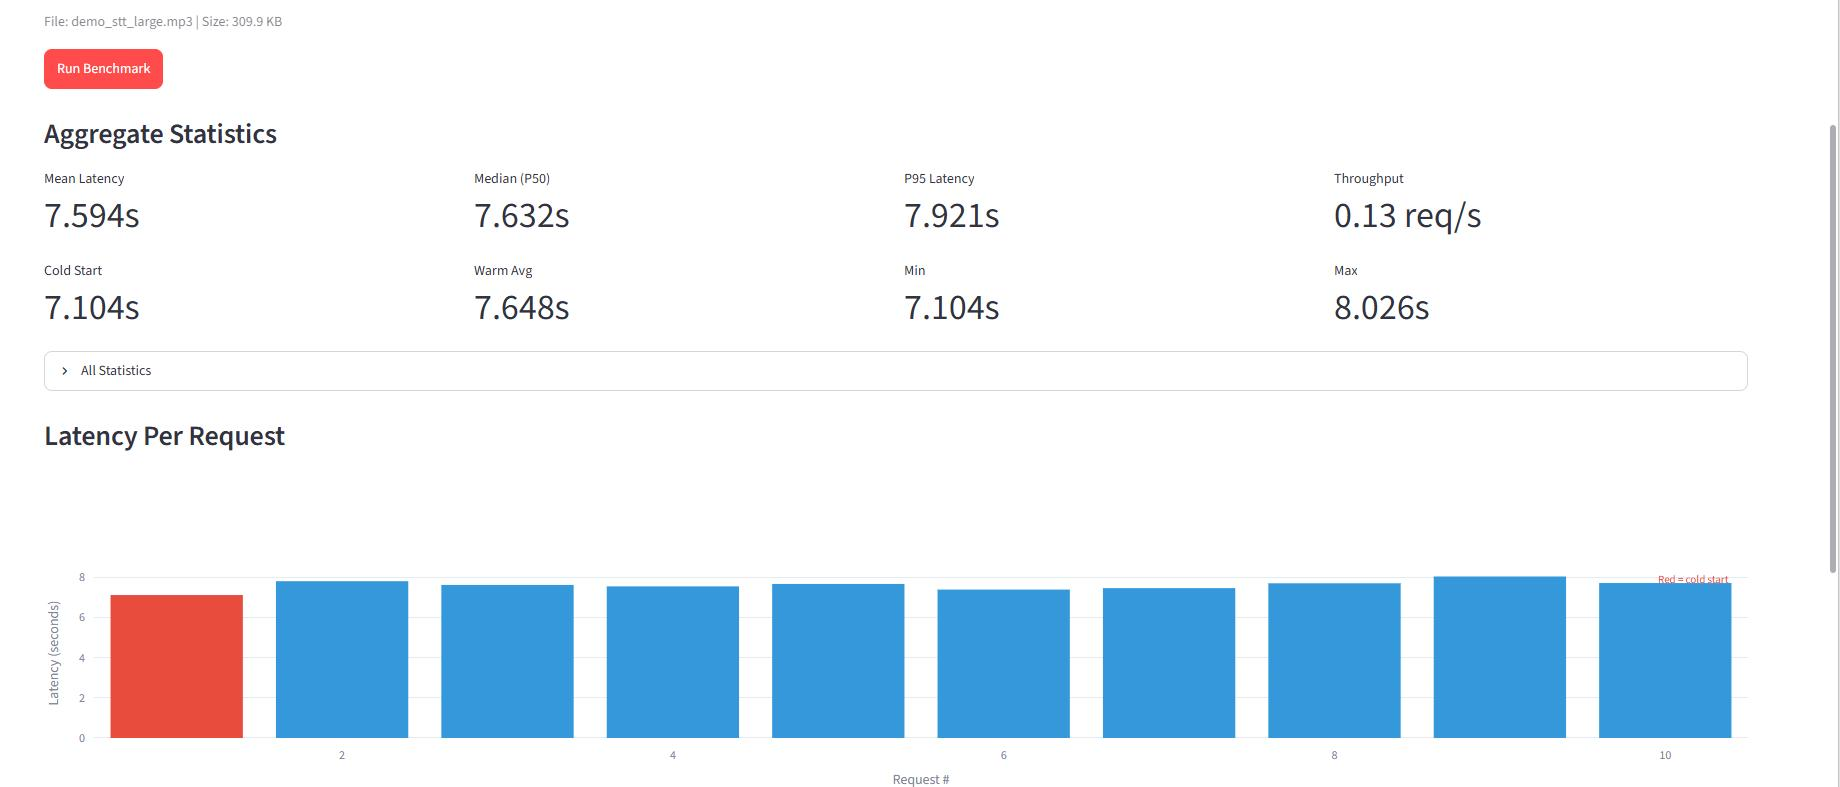
\includegraphics[width=0.9\textwidth]{../images/large/anh2.jpg}
    \caption{Kết quả benchmark -- file dài}
\end{figure}
\begin{figure}[H]
    \centering
    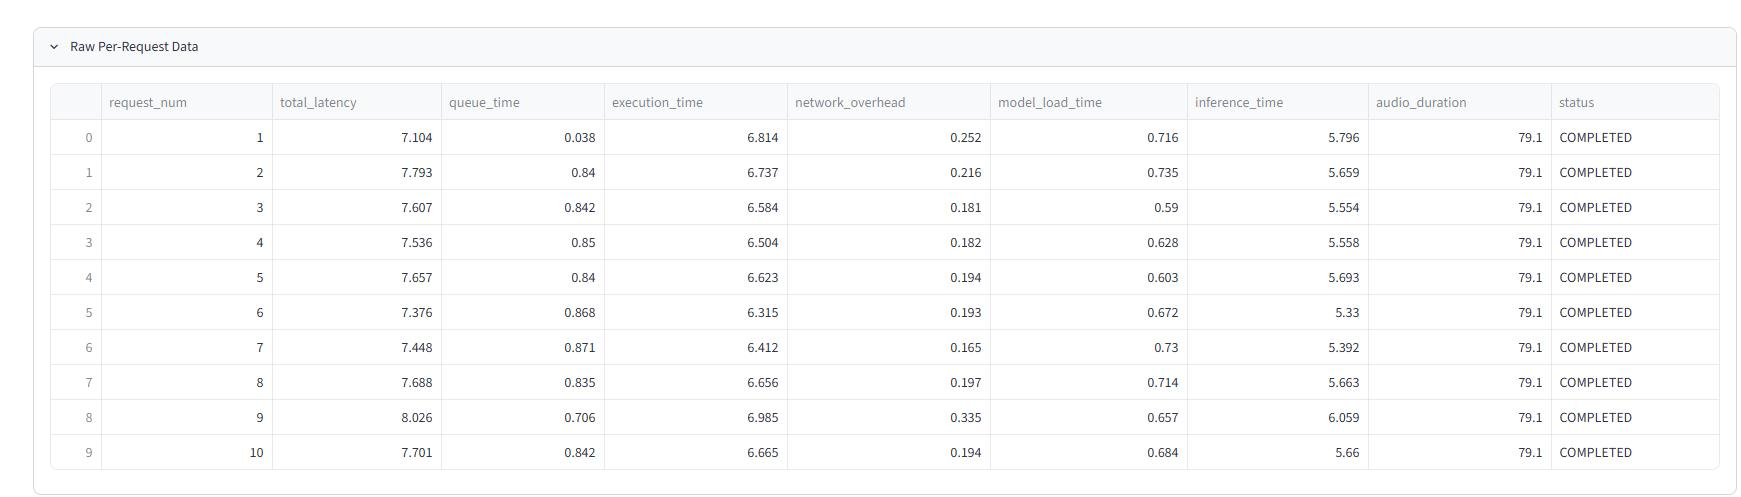
\includegraphics[width=0.9\textwidth]{../images/large/anh3.jpg}
    \caption{Dữ liệu thô từng request -- file dài}
\end{figure}
\begin{figure}[H]
    \centering
    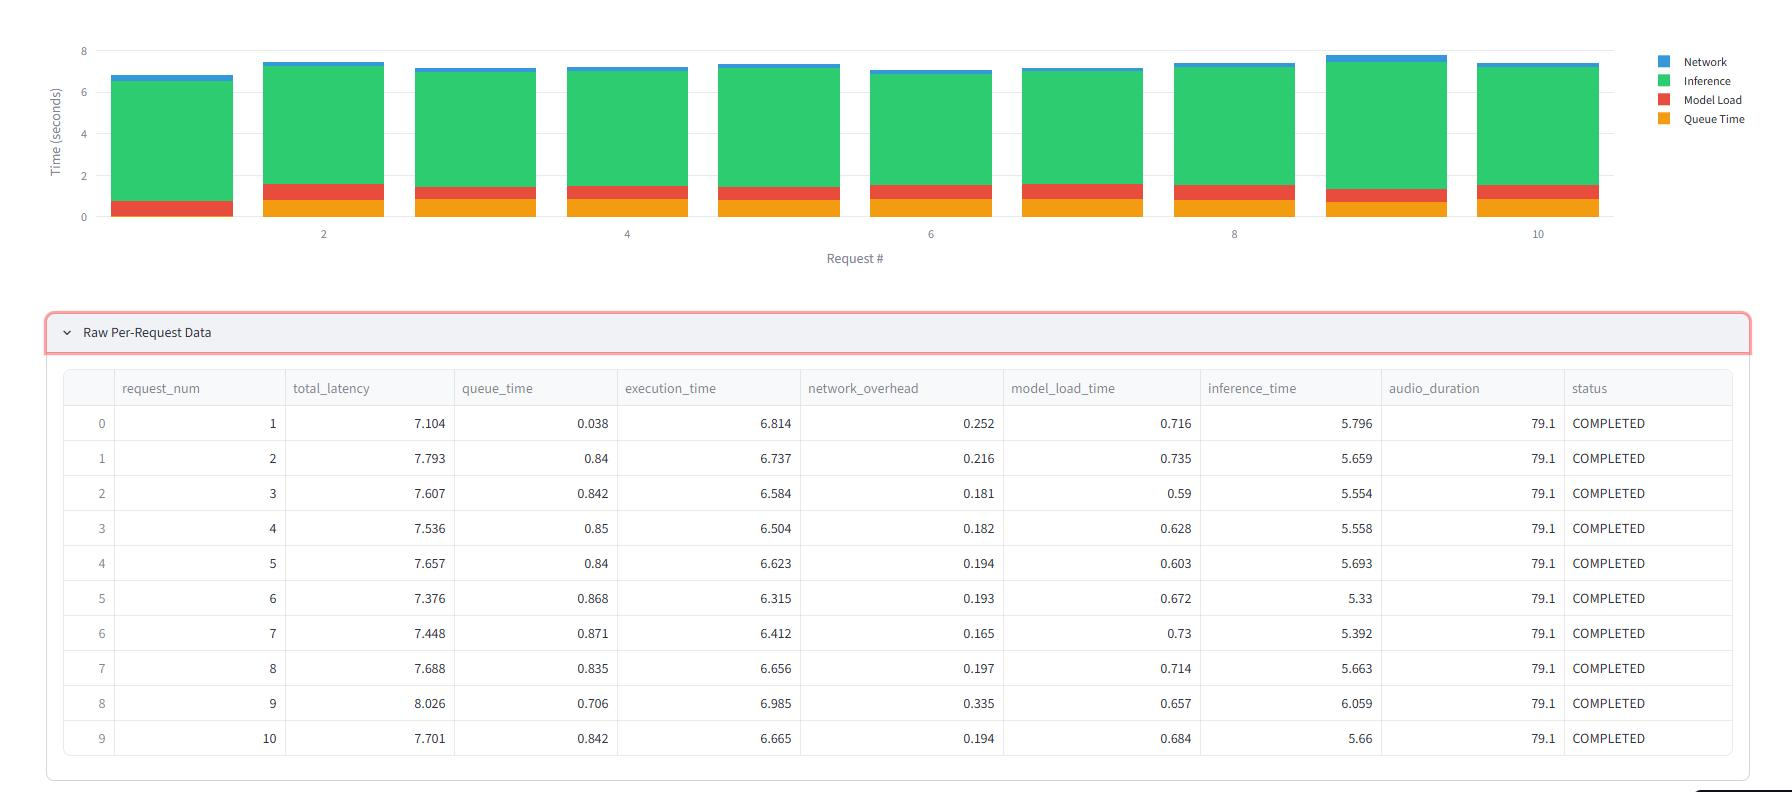
\includegraphics[width=0.9\textwidth]{../images/large/anh4.jpg}
    \caption{Biểu đồ phân bổ thời gian từng request -- file dài}
\end{figure}

\subsubsection{Kết quả request đơn lẻ}

\begin{table}[H]
\centering
\begin{tabular}{lr}
\toprule
\textbf{Chỉ số} & \textbf{Giá trị} \\
\midrule
Total Latency (end-to-end) & 6.993s \\
Queue Time & 0.020s \\
Execution Time & 6.743s \\
Network Overhead & 0.230s \\
\midrule
Model Load & 0.790s \\
Inference Only & 5.639s \\
Realtime Factor (RTF) & 0.07x \\
\bottomrule
\end{tabular}
\caption{Latency breakdown -- file dài, single request}
\end{table}

Dù file audio dài gấp 5 lần so với kịch bản 1, RTF vẫn giữ ở mức 0.07x -- cho thấy GPU A5000 không gặp tình trạng nghẽn khi xử lý chuỗi dữ liệu dài.

\subsubsection{Benchmark 10 requests liên tục}

\begin{table}[H]
\centering
\begin{tabular}{lr}
\toprule
\textbf{Chỉ số} & \textbf{Giá trị} \\
\midrule
Mean Latency & 7.594s \\
Median (P50) & 7.632s \\
P95 & 7.921s \\
Min / Max & 7.104s / 8.026s \\
\midrule
Cold Start & 7.104s \\
Warm Average & 7.648s \\
Throughput & 0.13 req/s \\
\bottomrule
\end{tabular}
\caption{Benchmark 10 requests -- file dài}
\end{table}

\subsubsection{Dữ liệu chi tiết từng request}

\begin{table}[H]
\centering
\small
\begin{tabular}{ccccccc}
\toprule
\textbf{\#} & \textbf{Total (s)} & \textbf{Queue (s)} & \textbf{Exec (s)} & \textbf{Network (s)} & \textbf{Load (s)} & \textbf{Infer (s)} \\
\midrule
1  & 7.104 & 0.038 & 6.814 & 0.252 & 0.716 & 5.796 \\
2  & 7.793 & 0.840 & 6.737 & 0.216 & 0.735 & 5.659 \\
3  & 7.607 & 0.842 & 6.584 & 0.181 & 0.590 & 5.554 \\
4  & 7.536 & 0.850 & 6.504 & 0.182 & 0.628 & 5.558 \\
5  & 7.657 & 0.840 & 6.623 & 0.194 & 0.603 & 5.693 \\
6  & 7.376 & 0.868 & 6.315 & 0.193 & 0.672 & 5.330 \\
7  & 7.448 & 0.871 & 6.412 & 0.165 & 0.730 & 5.392 \\
8  & 7.688 & 0.835 & 6.656 & 0.197 & 0.714 & 5.663 \\
9  & 8.026 & 0.706 & 6.985 & 0.335 & 0.657 & 6.059 \\
10 & 7.701 & 0.842 & 6.665 & 0.194 & 0.684 & 5.660 \\
\bottomrule
\end{tabular}
\caption{Dữ liệu chi tiết 10 requests -- file dài (79.1s audio)}
\end{table}



% ---------- Nhận xét ----------
\subsection{Nhận xét tổng hợp}

\begin{itemize}[noitemsep]
    \item RTF luôn dưới 0.1x ở cả hai kịch bản, tốc độ xử lý nhanh hơn thời gian thực ít nhất 10 lần.
    \item Độ lệch chuẩn thấp cho thấy thời gian phản hồi ổn định giữa các request, không suy giảm hiệu năng khi chạy liên tục.
    \item Cold Start chỉ ảnh hưởng ở request đầu tiên. Các request tiếp theo (warm) gần như không chênh lệch.
    \item Execution Time chiếm phần lớn tổng latency, Queue Time và Network Overhead rất nhỏ -- hạ tầng mạng của RunPod hoạt động ổn định.
\end{itemize}

% ==================== CHƯƠNG 2 ====================
\section{So sánh Kiến trúc Triển khai: RunPod Flash vs Docker Serverless}

Khi triển khai mô hình AI lên RunPod, có hai lựa chọn chính: sử dụng RunPod Flash (viết hàm Python kèm decorator \texttt{@Endpoint}) hoặc tự xây dựng Docker Image và deploy qua cơ chế Serverless truyền thống. Bảng dưới đây so sánh hai phương pháp dựa trên các tiêu chí vận hành thực tế.

\begin{table}[H]
\centering
\renewcommand{\arraystretch}{1.4}
\begin{tabularx}{\textwidth}{>{\raggedright\arraybackslash}p{3cm} X X}
\toprule
\textbf{Tiêu chí} & \textbf{RunPod Flash} & \textbf{Docker Serverless} \\
\midrule
Tốc độ deploy & Nhanh (vài giây). Chỉ cần gõ lệnh \texttt{flash deploy}. & Chậm hơn (vài phút). Cần build image, push lên registry, pull về server. \\
\midrule
Quản lý cấu hình & Viết trực tiếp trong code Python qua decorator \texttt{@Endpoint}. & Cấu hình trên Web UI hoặc qua API/Terraform riêng. \\
\midrule
Quản lý dependencies & Khai báo qua tham số \texttt{dependencies}, hệ thống tự cài đặt. & Toàn quyền kiểm soát thông qua \texttt{Dockerfile}. \\
\midrule
Tối ưu Cold Start & Cần tải model weights từ nguồn bên ngoài (HuggingFace, S3) mỗi lần worker khởi tạo lại. & Có thể đóng gói sẵn model weights vào Docker Image, giảm thời gian Cold Start. \\
\midrule
Kiểm soát version & Phụ thuộc vào base image nội bộ của RunPod. & Toàn quyền kiểm soát version thư viện, OS, CUDA driver. \\
\bottomrule
\end{tabularx}
\caption{So sánh RunPod Flash và Docker Serverless}
\end{table}

\subsection{Kết luận}

Dựa trên các đặc tính trên, đề xuất chia chiến lược triển khai thành hai giai đoạn:

\textbf{Giai đoạn R\&D và Testing -- nên dùng RunPod Flash.} Trong quá trình phát triển, team thường xuyên thử nghiệm nhiều model khác nhau (Whisper large-v2, v3, turbo) và thay đổi dependencies liên tục. RunPod Flash giúp giảm thiểu việc quản lý Docker image, tránh phải xử lý xung đột version giữa các lần thử nghiệm, cho phép team tập trung vào việc đánh giá model và demo kết quả nhanh.

\textbf{Giai đoạn Production -- nên dùng Docker Serverless.} Khi đã chốt được model và đưa vào phục vụ khách hàng thực tế, hệ thống cần tính ổn định cao và khả năng bảo trì lâu dài. Docker Serverless cho phép đóng gói cứng toàn bộ version thư viện và model weights thành một image duy nhất, giúp kiểm soát version chặt chẽ, đồng thời loại bỏ thời gian tải model qua mạng -- giảm đáng kể độ trễ Cold Start khi vận hành thực tế.

% ==================== CHƯƠNG 3 ====================
\section{Kiến trúc Multi-Model trên Serverless GPU (STT \& TTS)}

Dựa trên yêu cầu của hệ thống Voice Bot thực tế, chúng tôi đã nâng cấp kiến trúc RunPod Flash để xử lý đồng thời hai tác vụ: Nhận dạng giọng nói (Whisper STT) và Sinh giọng nói nhái giọng (XTTS-v2 Voice Cloning) trên \textbf{cùng một máy ảo GPU A5000}.

\subsection{Tối ưu không gian lưu trữ (Network Volume)}

Thay vì tải Model Weights từ internet mỗi khi có Cold Start (lên tới 3.7GB cho cả 2 model), toàn bộ weights được lưu trữ cố định trên \textbf{RunPod Network Volume}.
\begin{itemize}[noitemsep]
    \item \textbf{Giảm thiểu Cold Start:} Việc nạp model từ ổ cứng mạng SSD vào GPU VRAM (tốc độ ~300MB/s) giúp triệt tiêu hoàn toàn độ trễ tải mạng. Thời gian Cold Start cho cả 2 model giảm từ hơn 1 phút xuống chỉ còn \textbf{15-25 giây}.
    \item \textbf{Tối ưu gói triển khai:} Kích thước package code đẩy lên RunPod chỉ còn vài chục KB, giúp việc deploy diễn ra tức thời.
\end{itemize}

\subsection{Xử lý luồng (Routing) \& Batch Processing}

Để tiết kiệm chi phí, thay vì tách STT và TTS thành 2 API độc lập (khiến hệ thống phải duy trì 2 GPU riêng biệt), chúng tôi cấu hình \textbf{Unified Endpoint} nhận tham số \texttt{action="stt"} hoặc \texttt{action="tts"}. Hệ thống sử dụng Global Caching để giữ cả 2 model thường trực trong 24GB VRAM của A5000 (Whisper: $\sim$3GB, XTTS-v2: $\sim$2.1GB).

Đối với quá trình xử lý Batch cho STT, hệ thống áp dụng kỹ thuật \textbf{Server-Side Concurrency (GPU-level batching)} đạt chuẩn Production:
\begin{itemize}[noitemsep]
    \item Khởi tạo WhisperModel với \texttt{num\_workers=4}.
    \item Sử dụng \texttt{ThreadPoolExecutor} kết hợp CTranslate2 để đẩy nhiều file âm thanh vào GPU xử lý đồng thời trên các luồng CUDA độc lập.
    \item \textbf{Kết quả:} Cho phép xử lý cùng lúc nhiều phiên (sessions) hội thoại song song với hiệu năng vượt trội.
\end{itemize}

\end{document}
